%!Tex Root = ../Main.tex
% ./Packete_und_Deklarationen.tex
% ./Titlepage.tex
% ./Motivation.tex
% ./Einführung.tex
% ./Implementierung2_Pntr_Array.tex,
% ./Implementierung3_Struct_Derived.tex,
% ./Implementierung4_Fun.tex,
% ./Ergebnisse_und_Ausblick.tex

\chapter{Implementierung}
\label{ch:implementierung}

\section{Lexikalische Analyse}
\subsection{Teil der Konkretten Syntax für die Lexikalische Analyse}
\numberwithin{floatgrammar}{section}

\label{sec:lex_analyse_verwendung_von_lark}
% ./concrete_syntax_picoc.lark
\begin{grammar}[Teil der Konkretten Syntax der Sprache $L_{PicoC}$ für die Lexikalische Analyse in EBNF, Teil 1][H][gr:concrete_syntax_lex_teil_1]
  \toprule
  \firstcase{COMMENT}{\dq //\dq\enspace /[{\wedge}\backslash n]{*}/\gralt \dq {/*}\dq\enspace  /(.\mid \setminus n)*?/\enspace \dq {*/}\dq }{L\_Comment}
  \firstcase{RETI\_COMMENT.2}{\dq {//}\dq \dq \text{\textvisiblespace} \dq ? \dq \#\dq /[\wedge\backslash n]{*}/}{}
  \midrule
  \firstcase{DIG\_NO\_0}{\dq 1\dq \gralt \dq 2\dq \gralt \dq 3\dq \gralt \dq 4\dq \gralt \dq 5\dq}{L\_Arith}
  \otherform{\dq 6\dq \gralt \dq 7\dq \gralt \dq 8\dq \gralt \dq 9\dq}{}
  \firstcase{DIG\_WITH\_0}{\dq 0\dq \gralt DIG\_NO\_0}{}
  \firstcase{NUM}{\dq 0\dq \gralt DIG\_NO\_0 DIG\_WITH\_0*}{}
  \firstcase{ASCII\_CHAR}{\dq\text{\textvisiblespace} \dq ..\dq \sim\dq }{}
  \firstcase{CHAR}{\dq '\dq ASCII\_CHAR\dq '\dq }{}
  \firstcase{FILENAME}{ASCII\_CHAR+\dq .picoc\dq }{}
  \firstcase{LETTER}{\dq {a}\dq ..\dq {z}\dq \gralt \dq {A}\dq ..\dq {Z}\dq}{}
  \firstcase{NAME}{(LETTER\gralt \dq \_\dq )}{}
  & & \qquad(LETTER\gralt DIG\_WITH\_0\gralt \dq \_\dq )* & \\
  \firstcase{name}{NAME\gralt INT\_NAME\gralt CHAR\_NAME}{}
  \otherform{VOID\_NAME}{}
  \firstcase{NOT}{\dq \sim\dq }{}
  \firstcase{REF\_AND}{\dq \&\dq }{}
  \firstcase{un\_op}{SUB\_MINUS\gralt LOGIC\_NOT\gralt NOT}{}
  \otherform{MUL\_DEREF\_PNTR \gralt REF\_AND}{}
  \firstcase{MUL\_DEREF\_PNTR}{\dq {*}\dq }{}
  \firstcase{DIV}{\dq /\dq }{}
  \firstcase{MOD}{\dq \%\dq }{}
  \firstcase{prec1\_op}{MUL\_DEREF\_PNTR\gralt DIV\gralt MOD}{}
  \firstcase{ADD}{\dq {+}\dq }{}
  \firstcase{SUB\_MINUS}{\dq {-}\dq }{}
  \firstcase{prec2\_op}{ADD\gralt SUB\_MINUS}{}
  \midrule
  \firstcase{LT}{\dq {<}\dq }{L\_Logic}
  \firstcase{LTE}{\dq {<=}\dq }{}
  \firstcase{GT}{\dq {>}\dq }{}
  \firstcase{GTE}{\dq {>=}\dq }{}
  \firstcase{rel\_op}{LT\gralt LTE\gralt GT\gralt GTE}{}
  \firstcase{EQ}{\dq {==}\dq }{}
  \firstcase{NEQ}{\dq {!=}\dq }{}
  \firstcase{eq\_op}{EQ\gralt NEQ}{}
  \firstcase{LOGIC\_NOT}{\dq !\dq }{}
  \bottomrule
\end{grammar}

\begin{grammar}[Teil der Konkretten Syntax der Sprache $L_{PicoC}$ für die Lexikalische Analyse in EBNF, Teil 2][H][gr:concrete_syntax_lex_teil_2]
  \toprule
  \firstcase{INT\_DT.2}{\dq int\dq }{L\_Assign\_Alloc}
  \firstcase{INT\_NAME.3}{\dq int\dq\enspace (LETTER\gralt DIG\_WITH\_0\gralt \dq \_\dq )+}{}
  \firstcase{CHAR\_DT.2}{\dq char\dq }{}
  \firstcase{CHAR\_NAME.3}{\dq char\dq\enspace (LETTER\gralt DIG\_WITH\_0\gralt \dq \_\dq )+}{}
  \firstcase{VOID\_DT.2}{\dq void\dq }{}
  \firstcase{VOID\_NAME.3}{\dq void\dq\enspace (LETTER\gralt DIG\_WITH\_0\gralt \dq \_\dq )+}{}
  \firstcase{prim\_dt}{INT\_DT\gralt CHAR\_DT\gralt VOID\_DT}{}
  \bottomrule
\end{grammar}

% \begin{grammar}[\(\lambda\) calculus syntax][p][gr:ex1]
%   \firstcase{T}{\nonterm{V}}{Variable}
%   \otherform{(\nonterm{T}\ \nonterm{T})}{Application}
%   \otherform{\lambda \nonterm{V}\cdot\nonterm{T}}{Abstraction}
%   \firstcase{V}{x, y, \dots}{Variables}
% \end{grammar}
% \begin{grammar}[Advanced capabilities of \texttt{grammar.sty}][p][gr:ex2]
%   \firstcase{A}{\nonterm{T} \gralt \nonterm{V}}{Multiple option on a single line}
%   \highlight
%   \otherform{\nonterm{A}}{Highlighted form}
%   \downplay
%   \otherform{\nonterm{B}\gralt \nonterm{C}}{Downplayed form}
%   \otherform{\lochighlight{\nonterm{A}} \gralt \nonterm{B}}{Emphasize part of the line}
% \end{grammar}

% erwähnen, dass in Lark die Grammatiken L_Lex und L_Parse gemischt sind
% EBNF erwähnen
% (erwähnen, dass finalle Grammatik im Appendix)
\subsection{Basic Lexer}
\section{Syntaktische Analyse}
\label{sec:syntaktische_analyse}

\subsection{Teil der Konkretten Syntax für die Syntaktische Analyse}
% ./concrete_syntax_picoc.lark
% https://tex.stackexchange.com/questions/851/removing-spaces-between-words-in-math-mode
In \ref{gr:concrete_syntax_parser}

\begin{grammar}[Teil der Konkretten Syntax der Sprache $L_{PicoC}$ für die Syntaktische Analyse in EBNF, Teil 1][H][gr:concrete_syntax_parser]
  \toprule
	\downplay
  \firstcase{prim\_exp}{name\gralt NUM\gralt CHAR\gralt "("logic\_or")"}{L\_Arith +}
	\downplay
  \firstcase{post\_exp}{array\_subscr\gralt struct\_attr\gralt fun\_call}{L\_Array +}
	\downplay
  \otherform{input\_exp\gralt print\_exp\gralt prim\_exp}{L\_Pntr +}
	\downplay
  \firstcase{un\_exp}{un\_op un\_exp\gralt post\_exp}{L\_Struct + L\_Fun}
  \midrule
	\downplay
  \firstcase{input\_exp}{\dq input\dq\dq(\dq\dq)\dq}{L\_Arith}
	\downplay
  \firstcase{print\_exp}{\dq print\dq\dq(\dq logic\_or\dq)\dq}{}
	\downplay
  \firstcase{arith\_prec1}{arith\_prec1\enspace prec1\_op\enspace un\_exp\gralt un\_exp}{}
	\downplay
  \firstcase{arith\_prec2}{arith\_prec2\enspace prec2\_op\enspace arith\_prec1\gralt arith\_prec1}{}
	\downplay
  \firstcase{arith\_and}{arith\_and\enspace \dq\&\dq\enspace arith\_prec2\gralt arith\_prec2}{}
	\downplay
  \firstcase{arith\_oplus}{arith\_oplus\enspace \dq {\wedge{}}\dq\enspace arith\_and\gralt arith\_and}{}
	\downplay
  \firstcase{arith\_or}{arith\_or\enspace \dq{\mid} \dq\enspace arith\_oplus\gralt arith\_oplus}{}
  \midrule
  \downplay
  \firstcase{rel\_exp}{rel\_exp\enspace rel\_op\enspace arith\_or\gralt arith\_or}{L\_Logic}
  \downplay
  \firstcase{eq\_exp}{eq\_exp\enspace eq\_op rel\_exp\gralt rel\_exp}{}
  \downplay
  \firstcase{logic\_and}{logic\_and\enspace \dq{\&\&}\dq\enspace eq\_exp\gralt eq\_exp}{}
  \downplay
  \firstcase{logic\_or}{logic\_or\enspace \dq{\mid\mid}\dq\enspace logic\_and\gralt logic\_and}{}
  \midrule
	\downplay
  \firstcase{type\_spec}{prim\_dt\gralt struct\_spec}{L\_Assign\_Alloc}
	\downplay
  \firstcase{alloc}{type\_spec\enspace pntr\_decl}{}
	\downplay
  \firstcase{assign\_stmt}{un\_exp\enspace \dq {=}\dq\enspace logic\_or\dq ;\dq }{}
  \firstcase{initializer}{logic\_or\gralt array\_init\gralt struct\_init}{}
	\downplay
  \firstcase{init\_stmt}{alloc\enspace \dq {=}\dq\enspace initializer\dq ;\dq }{}
	\downplay
  \firstcase{const\_init\_stmt}{\dq const\dq\enspace type\_spec\enspace name\enspace \dq {=}\dq\enspace NUM\dq ;\dq }{}
  \midrule
  \firstcase{pntr\_deg}{\dq {*}\dq *}{L\_Pntr}
  \firstcase{pntr\_decl}{pntr\_deg\enspace array\_decl\gralt array\_decl}{}
  \midrule
  \firstcase{array\_dims}{(\dq [\dq NUM\dq ]\dq )*}{L\_Array}
  \firstcase{array\_decl}{name\enspace array\_dims\gralt \dq (\dq pntr\_decl\dq )\dq  array\_dims}{}
  \firstcase{array\_init}{\dq \{\dq initializer(\dq ,\dq\enspace initializer)*\dq \}\dq }{}
  \firstcase{array\_subscr}{post\_exp\dq [\dq logic\_or\dq ]\dq }{}
  \midrule
  \firstcase{struct\_spec}{\dq struct\dq\enspace name}{L\_Struct}
  \firstcase{struct\_params}{(alloc\dq ;\dq )+}{}
  \firstcase{struct\_decl}{\dq struct\dq\enspace name\enspace \dq \{\dq struct\_params\dq \}\dq }{}
  \firstcase{struct\_init}{\dq \{\dq \dq .\dq name\dq {=}\dq initializer}{}
  & & \qquad(\dq ,\dq\enspace \dq .\dq name\dq {=}\dq initializer)*\dq \}\dq & \\
  \firstcase{struct\_attr}{post\_exp\dq .\dq name}{}
  \midrule
	\downplay
  \firstcase{if\_stmt}{\dq if\dq \dq (\dq logic\_or\dq )\dq\enspace exec\_part}{L\_If\_Else}
	\downplay
  \firstcase{if\_else\_stmt}{\dq if\dq \dq (\dq logic\_or\dq )\dq\enspace exec\_part\enspace \dq else\dq\enspace exec\_part}{}
  \midrule
	\downplay
  \firstcase{while\_stmt}{\dq while\dq \dq (\dq logic\_or\dq )\dq\enspace exec\_part}{L\_Loop}
	\downplay
  \firstcase{do\_while\_stmt}{\dq do\dq\enspace exec\_part\enspace \dq while \dq \dq (\dq logic\_or\dq )\dq \dq ;\dq }{}
  \bottomrule
\end{grammar}

\begin{grammar}[Teil der Konkretten Syntax der Sprache $L_{PicoC}$ für die Syntaktische Analyse in EBNF, Teil 2][H]
  \toprule
	\downplay
  \firstcase{decl\_exp\_stmt}{alloc\dq ;\dq }{L\_Stmt}
	\downplay
  \firstcase{decl\_direct\_stmt}{ assign\_stmt\gralt init\_stmt\gralt const\_init\_stmt}{}
  \firstcase{decl\_part}{ decl\_exp\_stmt\gralt decl\_direct\_stmt\gralt RETI\_COMMENT}{}
  \\[-0.2cm]
	\downplay
  \firstcase{compound\_stmt}{ \dq \{\dq exec\_part* \dq \}\dq }{}
	\downplay
  \firstcase{exec\_exp\_stmt}{logic\_or\dq ;\dq }{}
	\downplay
  \firstcase{exec\_direct\_stmt}{if\_stmt\gralt if\_else\_stmt\gralt while\_stmt\gralt do\_while\_stmt}{}
	\downplay
  \otherform{assign\_stmt\gralt fun\_return\_stmt}{}
  \firstcase{exec\_part}{compound\_stmt\gralt exec\_exp\_stmt\gralt exec\_direct\_stmt}{}
  \otherform{RETI\_COMMENT}{}
  \\[-0.2cm]
  \firstcase{decl\_exec\_stmts}{decl\_part* exec\_part*}{}
  \midrule
  \firstcase{fun\_args}{[logic\_or(\dq ,\dq\enspace logic\_or)*]}{L\_Fun}
  \firstcase{fun\_call}{name\dq (\dq fun\_args\dq )\dq }{}
  \firstcase{fun\_return\_stmt}{\dq return\dq\enspace [logic\_or]\dq ;\dq }{}
  \firstcase{fun\_params}{[alloc(\dq ,\dq\enspace alloc)*]}{}
  \firstcase{fun\_decl}{type\_spec\enspace pntr\_deg\enspace name\dq (\dq fun\_params\dq )\dq }{}
  \firstcase{fun\_def}{type\_spec\enspace pntr\_deg\enspace name\dq (\dq fun\_params\dq )\dq\enspace \dq \{\dq  decl\_exec\_stmts \dq \}\dq }{}
  \midrule
  \firstcase{decl\_def}{(struct\_decl\gralt fun\_decl)\dq ;\dq \gralt fun\_def}{L\_File}
  \firstcase{decls\_defs}{decl\_def*}{}
  \firstcase{file}{FILENAME\enspace decls\_defs}{}
  \bottomrule
\end{grammar}
% Vorteile von Lark
\subsection{Umsetzung von Präzidenz}
Die \colorbold{PicoC} Programmiersprache hat dieselben \colorbold{Präzidenzregeln} implementiert, wie die Programmiersprache \colorbold{C} \footcite{noauthor_c_nodate}. Die \colorbold{Präzidenzregeln} von \colorbold{PicoC} sind in Tabelle~\ref{tab:reference_table} aufgelistet.

% \rowcolors{2}{SecondaryColor}{white}
\begin{table}[H]
  \center
  % \Block{2}{=}{Links, dann rechts $\rightarrow$} \\
  \begin{NiceTabular}{X[1,c]X[2,c]X[3,l]X[2,c]}[rules/color=PrimaryColor] % {\linewidth}{|C|C|L|L|}
  \CodeBefore
  \rowcolor{PrimaryColor}{1}
  \rowcolors{2-18}{SecondaryColor}{}[cols={2-3}]
  \rowcolors{2-18}{SecondaryColor}{}[cols={1,4}, respect-blocks, restart]
  \Body
  \textbf{\textcolor{white}{Präzidenz}} &	\textbf{\textcolor{white}{Operator}} & \textbf{\textcolor{white}{Beschreibung}} &	\textbf{\textcolor{white}{Assoziativität}} \\
  1	& \verb|a()|	& Funktionsaufruf & \Block{3-1}{Links, dann rechts $\rightarrow$} \\
    & \verb|a[]|	& Indexzugriff & \\
    & \verb|a.b| & Attributzugriff & \\
  2	&	\verb|-a| & Unäres Minus & \Block{3-1}{Rechts, dann links $\leftarrow$} \\
    & \smalltt{!a $\thicksim$a}	& Logisches NOT und Bitweise NOT & \\
    & \verb|*a &a| & Dereferenz und Referenz, auch Adresse-von & \\
  3	& \smalltt{a*b a/b a\%b} &	Multiplikation, Division und Modulo & \Block{9-1}{Links, dann rechts $\rightarrow$} \\
  4	& \verb|a+b a-b|	& Addition und Subtraktion & \\
  5	& \verb|a<b a<=b| \verb|a>b a>=b| & Kleiner, Kleiner Gleich, Größer, Größer gleich & \\
  6 &	\verb|a==b a!=b| & Gleichheit und Ungleichheit & \\
  7 &	\verb|a&b| & Bitweise UND & \\
  8 &	\verb|a^b| & Bitweise XOR (exclusive or) & \\
  9 & \smalltt{a$\mid$b} & Bitweise ODER (inclusive or) & \\
  10	& \verb|a&&b| &	Logiches UND & \\
  11	& $a{\mid\mid} b$	& Logisches ODER & \\
  12 & \verb|a=b| & Zuweisung & Rechts, dann links $\leftarrow$ \\
  13 &	\verb|a,b|& Komma	& Links, dann rechts $\rightarrow$ \\
  \bottomrule
\end{NiceTabular}
\caption{Präzidenzregeln von PicoC}
\label{tab:reference_table}
\end{table}
% erwähnen von Mehrdeutigkeit und Assoziativität
% finalle Grammatik im Appendix
% Crafting Compilers Quelle benennen

\subsection{Derivation Tree Generierung}
\subsubsection{Early Parser}
\subsubsection{Codebeispiel}
\label{sec:derivation_tree_generierung}
\begin{code}
  \centering
  \numberedcodebox[minted language=c]{./code_examples/example_dt_simple_ast_gen_array_decl_and_alloc.picoc}
  \caption{PicoC Code für Derivation Tree Generierung}
  \label{code:picoc_code_für_derivation_tree_generierung}
\end{code}

\begin{code}
  \centering
  \numberedcodebox[minted language=text]{./code_examples/example_dt_simple_ast_gen_array_decl_and_alloc.dt}
  \caption{Derivation Tree nach Derivation Tree Generierung}
  \label{code:derivation_tree_nach_derivation_tree_generierung}
\end{code}

\subsection{Derivation Tree Vereinfachung}
\subsubsection{Visitor}
\subsubsection{Codebeispiel}

Beispiel aus Subkapitel~\ref{sec:derivation_tree_generierung} wird fortgeführt.

\begin{code}
  \centering
  \numberedcodebox[minted language=text]{./code_examples/example_dt_simple_ast_gen_array_decl_and_alloc.dt_simple}
  \caption{Derivation Tree nach Derivation Tree Vereinfachung}
  \label{code:picoc_code_nach_derivation_tree_vereinfachung}
\end{code}

% Visitor erwähnen
\subsection{Abstrakt Syntax Tree Generierung}
\subsubsection{PicoC-Knoten}
% Tabelle aller PicoC Knoten
% möglichst kurze und leicht verständliche Bezeichner für Knoten

\begin{table}[H]
  \center
  \begin{NiceTabular}{X[7]X[10]}[rules/color=PrimaryColor]
  \CodeBefore
  \rowcolor{PrimaryColor}{1}
  \rowcolors{2-17}{SecondaryColor}{}[cols={1-2}]
  \Body
  \textbf{\textcolor{white}{PiocC-Knoten}} & \textbf{\textcolor{white}{Beschreibung}} \\
  \smalltt{Name(val)} & Ein \colorbold{Bezeichner}, z.B. \smalltt{my\_fun, my\_var} usw. , aber da es keine gute Kurzform für \smalltt{Identifier()} (englisches Wort für Bezeichner) gibt, wurde dieser Knoten \smalltt{Name()} genannt. \\
  \smalltt{Num(val)} & Eine \colorbold{Zahl}, z.B. \smalltt{42, -3} usw. \\
  \smalltt{Char(val)} & Ein \colorbold{Zeichen} der \colorbold{ASCII-Zeichenkodierung}, z.B. \smalltt{'c', '*'} usw. \\
  \smalltt{Minus(), Not(), DerefOp(), RefOp(), LogicNot()} & Die \colorbold{unären Operatoren} \smalltt{un\_op}: \smalltt{-a, {$\thicksim$}a, *a, \&a !a}. \\
  \smalltt{Add(), Sub(), Mul(), Div(), Mod(), Oplus(), And(), Or(), LogicAnd(), LogicOr()} & Die \colorbold{binären Operatoren} \smalltt{bin\_op}: \smalltt{a + b, a - b, a * b, a / b, a \% b, a $\wedge$ b, a \& b, a $\mid$ b, a \&\& b, a {$\mid\mid$} b}. \\
  \smalltt{Eq(), NEq(), Lt(), LtE(), Gt(), GtE()} & Die \colorbold{Relationen} \smalltt{rel}: \smalltt{a == b, a != b, a < b, a <= b, a > b, a >= b}. \\
  \smalltt{Const(), Writeable()} & Die \colorbold{Type Qualifier} \smalltt{type\_qual}: \smalltt{const}, was für ein \colorbold{nicht beschreibbare} \colorbold{Konstante} steht und das \colorbold{nicht} Angeben von \smalltt{const}, was für einen \colorbold{beschreibbare} Variable steht. \\
\smalltt{IntType(), CharType(), VoidType()} & Die \colorbold{Type Specifier} für \colorbold{Primitiven Datentypen}, die in der Abstrakten Syntax, um eine intuitive Bezeichnung zu haben einfach nur unter \colorbold{Datentypen} \smalltt{datatype} eingeordnet werden: \smalltt{int},  \smalltt{char},  \smalltt{void}. \\
\smalltt{Placeholder()} & \colorbold{Platzhalter} für einen Knoten, der diesen später \colorbold{ersetzt}. \\
  \smalltt{BinOp(exp, bin\_op, exp)} & Container für eine \colorbold{binäre Operation} mit $2$ Expressions: \smalltt{<exp1> <bin\_op> <exp2>}\\
  \smalltt{UnOp(un\_op, exp)} & Container für eine \colorbold{unäre Operation} mit einer Expression: \smalltt{<un\_op> <exp>}. \\
  \smalltt{Exit(num)} & Container für einen \colorbold{Exit Code}, der vor der Beendigung in das \smalltt{ACC} Register geschrieben wird und steht für die \colorbold{Beendigung} des laufenden Programmes. \\
  \smalltt{Atom(exp, rel, exp)} & Container für eine \colorbold{binäre Relation} mit $2$ Expressions: \smalltt{<exp1> <rel> <exp2>}\\
  \smalltt{ToBool(exp)} & Container für einen \colorbold{Arithmetischen Ausdruck}, wie z.B. \smalltt{1 + 3} oder einfach nur \smalltt{3}, der nicht nur $1$ oder $0$ als Ergebnis haben kann und daher bei einem Ergebnis $x > 1$ auf $1$ abgebildet wird. \\
  \smalltt{Alloc(type\_qual, datatype, name, \textcolor{gray!90!black}{local\_var\_or\_param})} & \colorbold{Container} für eine \colorbold{Allokation} \smalltt{<type\_qual> <datatype> <name>} mit den notwendigen Knoten \smalltt{type\_qual},  \smalltt{datatype} und  \smalltt{name}, die alle für einen Eintrag in der  \colorbold{Symboltabelle} notwendigen Informationen enthalten. Zudem besitzt er ein \textcolor{gray!90!black}{verstecktes Attribut}  \smalltt{local\_var\_or\_param}, dass die Information trägt, ob es sich bei der \colorbold{Variable} um eine \colorbold{Lokale Variable} oder einen \colorbold{Parameter} handelt. \\
  \smalltt{Assign(lhs, exp)} & Container für eine \colorbold{Zuweisung}, wobei \smalltt{lhs} ein  \smalltt{Subscr(exp1, exp2)}, \smalltt{Deref(exp1, exp2)}, \smalltt{Attr(exp, name)} oder  \smalltt{Name('var')} sein kann und  \smalltt{exp} ein beliebiger \colorbold{Logischer Ausdruck} sein kann: \smalltt{lhs = exp}. \\
  \bottomrule
\end{NiceTabular}
\caption{PicoC-Knoten Teil 1}
\label{tab:picoc_knoten_teil_1}
\end{table}

\begin{table}[H]
  \center
  \begin{NiceTabular}{X[7]X[10]}[rules/color=PrimaryColor]
  \CodeBefore
  \rowcolor{PrimaryColor}{1}
  \rowcolors{2-13}{SecondaryColor}{}[cols={1-2}]
  \Body
  \textbf{\textcolor{white}{PiocC-Knoten}} & \textbf{\textcolor{white}{Beschreibung}} \\
  \smalltt{Exp(exp, \textcolor{gray!90!black}{datatype}, \textcolor{gray!90!black}{error\_data})} & Container für einen \colorbold{beliebigen Ausdruck}, dessen Ergebnis auf den \colorbold{Stack} soll. Zudem besitzt er $2$ \textcolor{gray!90!black}{versteckte Attribute}, wobei \smalltt{datatype} im \colorbold{RETI Blocks Pass} wichtig ist und \smalltt{error\_data} für \colorbold{Fehlermeldungen} wichtig ist. \\
  \smalltt{Stack(num)} & Container, der für das \colorbold{temporäre} Ergebnis einer Berechnung, das \smalltt{num} Speicherzellen relativ zum  \colorbold{Stackpointer Register} \smalltt{SP} steht.\\
  \smalltt{Stackframe(num)} & Container, der für eine Variable steht, die \smalltt{num} Speicherzellen relativ zum \colorbold{Begin-Aktive-Funktion Register} \smalltt{BAF} steht. \\
  \smalltt{Global(num)} & Container, der für eine Variable steht, die \smalltt{num} Speicherzellen relativ zum \colorbold{Datensegment Register} \smalltt{DS} steht. \\
  \smalltt{StackMalloc(num)} & Container, der für das \colorbold{Allokieren} von \smalltt{num} Speicherzellen auf dem \colorbold{Stack} steht. \\
\smalltt{PntrDecl(num, datatype)} & Container, der für den \colorbold{Pointerdatentyp} steht: \smalltt{<prim\_dt> *<var>}, wobei das \colorbold{Attribut} \smalltt{num} die \colorbold{Anzahl zusammengefasster Pointer} angibt und \smalltt{datatype} der {Datentyp} ist, auf den der oder die \colorbold{Pointer} zeigen. \\
\smalltt{Ref(exp, \textcolor{gray!90!black}{datatype}, \textcolor{gray!90!black}{error\_data})} & Container, der für die Anwendung des \colorbold{Referenz-Operators} \smalltt{\&<var>} steht und die \colorbold{Adresse} einer \colorbold{Location} (Definition~\ref{def:location}) auf den Stack schreiben soll, die über \smalltt{exp} eingegrenzt wird. Zudem besitzt er $2$ \textcolor{gray!90!black}{versteckte Attribute}, wobei \smalltt{datatype} im \colorbold{RETI Blocks Pass} wichtig ist und \smalltt{error\_data} für \colorbold{Fehlermeldungen} wichtig ist. \\
\smalltt{Deref(lhs, exp)} & Container für den \colorbold{Indexzugriff} auf einen \colorbold{Array-} oder \colorbold{Pointerdatentyp}: \smalltt{<var>[<i>]}, wobei \smalltt{exp1} eine angehängte weitere \smalltt{Subscr(exp1, exp2)}, \smalltt{Deref(exp1, exp2)}, \smalltt{Attr(exp, name)} oder ein \smalltt{Name('var')} sein kann und \smalltt{exp2} der Index ist auf den zugegriffen werden soll. \\
\smalltt{ArrayDecl(nums, datatype)} & Container, der für den \colorbold{Arraydatentyp} steht: \smalltt{<prim\_dt> <var>[<i>]}, wobei das \colorbold{Attribut} \smalltt{nums} eine Liste von \smalltt{Num('x')} ist, die die \colorbold{Dimensionen} des Arrays angibt und \smalltt{datatype} der {Datentyp} ist, der über das Anwenden von \smalltt{Subscript()} auf das Array zugreifbar ist. \\
\smalltt{Array(exps, \textcolor{gray!90!black}{datatype})} & Container für den \colorbold{Initializer} eines \colorbold{Arrays}, dessen Einträge \smalltt{exps} weitere Initializer für eine \colorbold{Array-Dimension} oder ein Initializer für ein \colorbold{Struct} oder ein \colorbold{Logischer Ausdruck} sein können, z.B. \smalltt{\{\{1, 2\}, \{3, 4\}\}}. Des Weiteren besitzt er ein \textcolor{gray!90!black}{verstecktes Attribut} \smalltt{datatype}, welches für den \colorbold{PicoC-Mon Pass} Informationen transportiert, die für \colorbold{Fehlermeldungen} wichtig sind. \\
\smalltt{Subscr(exp1, exp2)} & Container für den \colorbold{Indexzugriff} auf einen \colorbold{Array-} oder \colorbold{Pointerdatentyp}: \smalltt{<var>[<i>]}, wobei \smalltt{exp1} eine angehängte weitere \smalltt{Subscr(exp1, exp2)}, \smalltt{Deref(exp1, exp2)} oder \smalltt{Attr(exp, name)} Operation sein kann oder ein \smalltt{Name('var')} sein kann und \smalltt{exp2} der Index ist auf den zugegriffen werden soll. \\
  \smalltt{StructSpec(name)} & Container für einen selbst definierten \colorbold{Structdatentyp}: \smalltt{struct <name>}, wobei das \colorbold{Attribut} \smalltt{name} festlegt, welchen \colorbold{selbst definierte} Structdatentyp dieser Container-Knoten repräsentiert. \\
  \smalltt{Attr(exp, name)} & Container für den \colorbold{Attributzugriff} auf einen \colorbold{Structdatentyp}: \smalltt{<var>.<attr>}, wobei \smalltt{exp1} eine angehängte weitere \smalltt{Subscr(exp1, exp2)}, \smalltt{Deref(exp1, exp2)} oder \smalltt{Attr(exp, name)} Operation sein kann oder ein \smalltt{Name('var')} sein kann und \smalltt{name} das Attribut ist, auf das zugegriffen werden soll. \\
  \bottomrule
\end{NiceTabular}
\caption{PicoC-Knoten Teil 2}
\label{tab:picoc_knoten_teil_2}
\end{table}

\begin{table}[H]
  \center
  \begin{NiceTabular}{X[7]X[10]}[rules/color=PrimaryColor]
  \CodeBefore
  \rowcolor{PrimaryColor}{1}
  \rowcolors{2-9}{SecondaryColor}{}[cols={1-2}]
  \Body
  \textbf{\textcolor{white}{PiocC-Knoten}} & \textbf{\textcolor{white}{Beschreibung}} \\
  \smalltt{Struct(assigns, \textcolor{gray!90!black}{datatype})} & Container für den \colorbold{Initializer} eines \colorbold{Structs}, z.B \smalltt{\{.<attr1>=\{1, 2\}, .<attr2>=\{3, 4\}\}}, dessen Eintrag \smalltt{assigns} eine Liste von \smalltt{Assign(lhs, exp)} ist mit einer Zuordnung eines \colorbold{Attributezeichners}, zu einem weiteren Initializer für eine \colorbold{Array-Dimension} oder zu einem Initializer für ein \colorbold{Struct} oder zu einem \colorbold{Logischen Ausdruck}. Des Weiteren besitzt er ein  \textcolor{gray!90!black}{verstecktes Attribut} \smalltt{datatype}, welches für den \colorbold{PicoC-Mon Pass} Informationen transportiert, die für \colorbold{Fehlermeldungen} wichtig sind. \\
  \smalltt{StructDecl(name, allocs)} & Container für die Deklaration eines \colorbold{selbstdefinierten Structdatentyps}, z.B. \smalltt{struct <var> \{<datatype> <attr1>; <datatype> <attr2>;\};}, wobei \smalltt{name} der \colorbold{Bezeichner} des Structdatentyps ist und \smalltt{allocs} eine Liste von Bezeichnern der \colorbold{Attribute} des Structdatentyps mit dazugehörigem \colorbold{Datentyp}, wofür sich der \colorbold{Container-Knoten} \smalltt{Alloc(type\_qual, datatype, name)} sehr gut als \colorbold{Container} eignet. \\
  \smalltt{If(exp, stmts)} & Container für ein \colorbold{If Statement} \smalltt{if(<exp>) \{ <stmts> \}} inklusive  \colorbold{Condition}  \smalltt{exp} und einem  \colorbold{Branch}  \smalltt{stmts}, indem eine \colorbold{Liste von Statements} stehen kann oder ein einzelnes \smalltt{GoTo(Name('block.xyz'))}. \\
  \smalltt{IfElse(exp, stmts1, stmts2)} & Container für ein \colorbold{If-Else Statement} \smalltt{if(<exp>) \{ <stmts2> \} else \{ <stmts2> \}} inklusive \colorbold{Codition} \smalltt{exp} und $2$ \colorbold{Branches} \smalltt{stmts1} und \smalltt{stmts2}, die zwei Alternativen Darstellen in denen jeweils \colorbold{Listen von Statements} oder  \smalltt{GoTo(Name('block.xyz'))}'s stehen können. \\
  \smalltt{While(exp, stmts)} & Container für ein \colorbold{While-Statement} \smalltt{while(<exp>) \{ <stmts> \}} inklusive  \colorbold{Condition}  \smalltt{exp} und einem \colorbold{Branch}  \smalltt{stmts}, indem eine \colorbold{Liste von Statements} stehen kann oder ein einzelnes \smalltt{GoTo(Name('block.xyz'))}. \\
  \smalltt{DoWhile(exp, stmts)} & Container für ein \colorbold{Do-While-Statement} \smalltt{do \{ <stmts> \} while(<exp>);} inklusive  \colorbold{Condition}  \smalltt{exp} und einem \colorbold{Branch}  \smalltt{stmts}, indem eine \colorbold{Liste von Statements} stehen kann oder ein einzelnes \smalltt{GoTo(Name('block.xyz'))}. \\
  \smalltt{Call(name, exps)} & Container für einen \colorbold{Funktionsaufruf}: \smalltt{fun\_name(exps)}, wobei \smalltt{name} der \colorbold{Bezeichner} der Funktion ist, die aufgerufen werden soll und \smalltt{exps} eine \colorbold{Liste von Argumenten} ist, die an die Funktion übergeben werden soll. \\
  \smalltt{Return(exp)} & Container für ein \smalltt{Return-Statement}: \smalltt{return <exp>}, wobei das  \colorbold{Attribut}  \smalltt{exp} einen  \colorbold{Logischen Ausdruck} darstellt, dessen Ergebnis vom  \colorbold{Return-Statement} zurückgegeben wird. \\
  \smalltt{FunDecl(datatype, name, allocs)} & Container für eine \colorbold{Funktionsdeklaration}, z.B. \smalltt{<datatype> <fun\_name>(<datatype> <param1>, <datatype> <param2>)}, wobei \smalltt{datatype} der  \colorbold{Rückgabewert} der Funktion ist,  \smalltt{name} der  \colorbold{Bezeichner} der Funktion ist und \smalltt{allocs} die \colorbold{Parameter} der Funktion sind, wobei der \colorbold{Container-Knoten} \smalltt{Alloc(type\_spec, datatype, name)} als Cotainer für die Parameter dient. \\
  \bottomrule
\end{NiceTabular}
\caption{PicoC-Knoten Teil 3}
\label{tab:picoc_knoten_teil_3}
\end{table}

\begin{table}[H]
  \center
  \begin{NiceTabular}{X[7]X[10]}[rules/color=PrimaryColor]
  \CodeBefore
  \rowcolor{PrimaryColor}{1}
  \rowcolors{2-9}{SecondaryColor}{}[cols={1-2}]
  \Body
  \textbf{\textcolor{white}{PiocC-Knoten}} & \textbf{\textcolor{white}{Beschreibung}} \\
  \smalltt{FunDef(datatype, name, allocs, stmts\_blocks)} & Container für eine \colorbold{Funktionsdefinition}, z.B. \smalltt{<datatype> <fun\_name>(<datatype> <param>) \{<stmts>\}}, wobei \smalltt{datatype} der  \colorbold{Rückgabewert} der Funktion ist,  \smalltt{name} der  \colorbold{Bezeichner} der Funktion ist, \smalltt{allocs} die \colorbold{Parameter} der Funktion sind, wobei der \colorbold{Container-Knoten} \smalltt{Alloc(type\_spec, datatype, name)} als Cotainer für die Parameter dient und \smalltt{stmts\_blocks} eine Liste von \colorbold{Statemetns} bzw.  \colorbold{Blöcken} ist, welche diese Funktion beinhaltet. \\
  \smalltt{NewStackframe(fun\_name, goto\_after\_call)} & Container für die \colorbold{Erstellung} eines neuen \colorbold{Stackframes} und Speicherung des Werts des \smalltt{BAF}-Registers der \colorbold{aufrufenden Funktion} und der \colorbold{Rücksprungadresse} nacheinander an den \colorbold{Anfang} des neuen \colorbold{Stackframes}. Das Attribut \smalltt{fun\_name} stehte dabei für den Bezeichner der Funktion, für die ein neuer \colorbold{Stackframe} erstellt werden soll. Das Attribut \smalltt{fun\_name} dient später dazu den \colorbold{Block} dieser Funktion zu finden, weil dieser für den weiteren Kompiliervorang wichtige Information in seinen \textcolor{gray!90!black}{versteckte Attributen} gespeichert hat. Des Weiteren ist das Attribut \smalltt{goto\_after\_call} ein \smalltt{GoTo(Name('addr@next\_instr'))}, welches später durch die \colorbold{Adresse} des Befehls, der direkt auf die \colorbold{Jump Instruction} folgt, ersetzt wird.\\
  \smalltt{RemoveStackframe()} & Container für das \colorbold{Entfernen} des aktuellen \colorbold{Stackframes} durch das \colorbold{Wiederherstellen} des im noch \colorbold{aktuellen Stackframe} gespeicherten Werts des \smalltt{BAF}-Registes der \colorbold{aufrufenden Funktion} und das Setzen des \smalltt{SP}-Registers auf den Wert des \smalltt{BAF}-Registesr \colorbold{vor} der Wiederherstellung. \\
  \smalltt{File(name, decls\_defs\_blocks)} & Container für alle \colorbold{Funkionen} oder \colorbold{Blöcke}, welche eine Datei als Ursprung haben, wobei \smalltt{name} der \colorbold{Dateiname} der Datei ist, die erstellt wird und \smalltt{decls\_defs\_blocks} eine Liste von \colorbold{Funktionen} bzw. \colorbold{Blöcken} ist. \\
  \smalltt{Block(name, stmts\_instrs, \textcolor{gray!90!black}{instrs\_before}, \textcolor{gray!90!black}{num\_instrs}, \textcolor{gray!90!black}{param\_size}, \textcolor{gray!90!black}{local\_vars\_size})} & Container für \colorbold{Statements}, der auch als \colorbold{Block} bezeichnet wird, wobei das Attribut \smalltt{name} der Bezeichners des \colorbold{Labels} (Definition~\ref{def:label}) des Blocks ist und \smalltt{stmts\_instrs} eine \colorbold{Liste von Statements} oder \colorbold{Instructions}. Zudem besitzt er noch $3$ \textcolor{gray!90!black}{versteckte Attribute}, wobei  \smalltt{instrs\_before} die Zahl der \colorbold{Instructions} vor diesem \colorbold{Block} zählt,  \smalltt{num\_instrs} die Zahl der Instructions ohne Kommentare in diesem Block zählt, \smalltt{param\_size} die voraussichtliche Anzahl an Speicherzellen aufaddiert, die für die \colorbold{Parameter} der Funktion belegt werden müssen und \smalltt{local\_vars\_size} die voraussichtliche Anzahl an Speicherzellen aufaddiert, die für die \colorbold{lokalen Variablen} der Funktion belegt werden müssen. \\
  \smalltt{GoTo(name)} & Container für ein \smalltt{Goto} zu einem anderen \colorbold{Block}, wobei das Attribut \smalltt{name} der Bezeichner des \colorbold{Labels} des Blocks ist zu dem Gesprungen werden soll. \\
  \smalltt{SingleLineComment(prefix, content)} & Container für einen \colorbold{Kommentar}, den der Compiler selber während des \colorbold{Kompiliervorangs} erstellt, der im \colorbold{RETI-Interpreter} selbst später \colorbold{nicht} sichtbar sein wird, aber in den \colorbold{Immediate}-Dateien, welche die \colorbold{Abstract Syntax Trees} nach den verschiedenen \colorbold{Passes} enthalten. \\
  \smalltt{RETIComment(value)} & Container für einen \colorbold{Kommentar} im Code der Form: \smalltt{// \# comment}, der im \colorbold{RETI-Intepreter} später sichtbar sein wird und zur Orientierung genutzt werden kann, allerdings in einer tatsächlichen Implementierung einer \colorbold{RETI-CPU} \colorbold{nicht umsetzbar} ist und auch nicht sinnvoll wäre umzusetzen. Der \colorbold{Kommentar} ist im Attribut \colorbold{value}, welches jeder Knoten besitzt gespeichert. \\
  \bottomrule
\end{NiceTabular}
\caption{PicoC-Knoten Teil 4}
\label{tab:picoc_knoten_teil_4}
\end{table}


\begin{Definition}{Label}{label}
  Durch einen \colorbold{Bezeichner} \colorbold{eindeutig} zuordenbares \colorbold{Sprungziel} im Programmcode.\footcite{thiemann_compilerbau_2021}
\end{Definition}

\begin{Definition}{Location}{location}
  Kollektiver Begriff für \colorbold{Variablen}, \colorbold{Attribute} bzw. \colorbold{Elemente} von Variablen bestimmter Datentypen, \colorbold{Speicherbereiche auf dem Stack}, die \colorbold{temporäre Zwischenergebnisse} speichern und \colorbold{Register}.

  Im Grunde genommen alles, was mit einem \colorbold{Programm zu tuen} hat und irgendwo \colorbold{gespeichert} ist.\footcite{g_siek_course_2022}
\end{Definition}

\begin{Special_Paragraph}
  Die \textcolor{gray!90!black}{ausgegrauten} Attribute der PicoC-Nodes sind \textcolor{gray!90!black}{versteckte Attribute}, die \colorbold{nicht} direkt bei der Erstellung der  \colorbold{PicoC-Nodes} mit einem Wert \colorbold{initialisiert} werden, sondern im \colorbold{Verlauf der Kompilierung} beim Durchlaufen der verschiedenen Passes etwas zugewiesen bekommen, dass im weiteren Kompiliervorgang \colorbold{Informationen} transportiert, die später im Kompiliervorgang nicht mehr so leicht zugänglich wären.

  Jeder \colorbold{Knoten} hat darüberhinaus auch noch $2$ \colorbold{Attribute} \smalltt{value} und \smalltt{position}, wobei \colorbold{value} bei einem \colorbold{Token-Knoten} (Definition~\ref{def:token_knoten}) dem \colorbold{Tokenwert} des Tokens, welches es ersetzt entspricht und bei \colorbold{Container-Knoten} (Definition~\ref{def:container_knoten}) unbesetzt ist. Das \colorbold{Attribut} \smalltt{position} wird später für Fehlermeldungen gebraucht.
\end{Special_Paragraph}

\begin{Definition}{Token-Knoten}{token_knoten}
  Ersetzt ein \colorbold{Token} bei der Generierung des \colorbold{Abstract Syntax Tree}, damit der Zugriff auf Knoten des Abstract Syntax Tree möglichst \colorbold{simpel} ist und keine vermeidbaren Fallunterscheidungen gemacht werden müssen.

  \colorbold{Token-Knoten} entsprechen im Abstract Syntax Tree \colorbold{Blättern}.\footcite{thiemann_compilerbau_2021}
\end{Definition}

\begin{Definition}{Container-Knoten}{container_knoten}
  Dient als \colorbold{Container} für andere \colorbold{Container-Knoten} und \colorbold{Token-Knoten}. Die \colorbold{Container-Knoten} werden optimalerweise immer so gewählt, dass sie \colorbold{mehrere Produktionen} der \colorbold{Konkretten Syntax} abdecken, die einen \colorbold{gleichen Aufbau} haben und sich auch unter einem \colorbold{Überbegriff} zusammenfassen lassen.\footnote{Wie z.B. die verschiedenen \colorbold{Arithmetischen Ausdrücke}, wie z.B. \smalltt{1 {\%} 3} und \colorbold{Logischen Ausdrücke}, wie z.B. \smalltt{1 \&\& 2 < 3}, die einen gleichen Aufbau haben mit immer einer \colorbold{Operation} in der Mitte haben und $2$ \colorbold{Operanden} auf beiden Seiten und sich unter dem Überbegriff \colorbold{Binäre Operationen} zusammenfassen lassen.}

  \colorbold{Container-Knoten} entsprechen im Abstract Syntax Tree \colorbold{Inneren Knoten}.\footcite{thiemann_compilerbau_2021}
\end{Definition}

\subsubsection{RETI-Knoten}
\begin{table}[H]
  \center
  \begin{NiceTabular}{X[8]X[10]}[rules/color=PrimaryColor]
  \CodeBefore
  \rowcolor{PrimaryColor}{1}
  \rowcolors{2-16}{SecondaryColor}{}[cols={1-2}]
  \Body
  \textbf{\textcolor{white}{RETI-Knoten}} &	\textbf{\textcolor{white}{Beschreibung}} \\
  \smalltt{Program(name, instrs)} & Container für alle \colorbold{Instructions}: \smalltt{<name> <instrs>}, wobei \smalltt{name} der \colorbold{Dateiname} der Datei ist, die erstellt wird und \smalltt{instrs} eine \colorbold{Liste von Instructions} ist. \\
  \smalltt{Instr(op, args)} & Container für eine \colorbold{Instruction}: \smalltt{<op> <args>}, wobei \smalltt{op} eine \colorbold{Operation} ist und  \smalltt{args} eine \colorbold{Liste von Argumenten} für dieser Operation. \\
  \smalltt{Jump(rel, im\_goto)} & Container für eine \colorbold{Jump-Instruction}: \smalltt{JUMP<rel> <im>}, wobei \smalltt{rel} eine \colorbold{Relation} ist und \smalltt{im\_goto} ein \colorbold{Immediate Value} \smalltt{Im(val)} für die \colorbold{Anzahl an Speicherzellen}, um die relativ zur \colorbold{Jump-Instruction} gesprungen werden soll oder ein \smalltt{GoTo(Name('block.xyz'))}, das später im \colorbold{RETI-Patch Pass} durch einen passenden \colorbold{Immediate Value} ersetzt wird. \\
  \smalltt{Int(num)} & Container für einen \colorbold{Interruptaufruf}: \smalltt{INT <im>}, wobei \smalltt{num} die \colorbold{Interrruptvektornummer} (IVN) für die passende Speicherzelle in der \colorbold{Interruptvektortabelle} ist, in der die Adresse der \colorbold{Interrupt-Service-Routine} (ISR) steht. \\
  \smalltt{Call(name, reg)} & Container für einen \colorbold{Prozeduraufruf}: \smalltt{CALL <name> <reg>}, wobei \smalltt{name} der \colorbold{Bezeichner} der  Prozedur, die aufgerufen werden soll ist und \smalltt{reg} ein \colorbold{Register} ist, das als \colorbold{Argument} an die Prozedur dient. Diese \colorbold{Operation} ist in der Betriebssysteme Vorlesung\tabularnote{\cite{scholl_betriebssysteme_2020}} nicht deklariert, sondern wurde dazuerfunden, um unkompliziert ein  \smalltt{CALL PRINT ACC} oder  \smalltt{CALL INPUT ACC} im RETI-Interpreter simulieren zu können. \\
  \smalltt{Name(val)} & Bezeichner für eine \colorbold{Prozedur}, z.B. \smalltt{PRINT} oder \smalltt{INPUT} oder den \colorbold{Programnamen}, z.B. \smalltt{PROGRAMNAME}. Dieses \colorbold{Argument} ist in der Betriebssysteme Vorlesung\tabularnote{\cite{scholl_betriebssysteme_2020}} nicht deklariert, sondern wurde dazuerfunden, um Bezeichner, wie \smalltt{PRINT}, \smalltt{INPUT} oder \smalltt{PROGRAMNAME} schreiben zu können. \\
  \smalltt{Reg(reg)} & Container für ein \colorbold{Register}. \\
  \smalltt{Im(val)} & Ein \colorbold{Immediate Value}, z.B. \smalltt{42, -3} usw. \\
  \smalltt{Add(), Sub(), Mult(), Div(), Mod(), Oplus(), Or(), And()} & \colorbold{Compute-Memory} oder \colorbold{Compute-Register} Operationen: \smalltt{ADD, SUB, MULT, DIV, OPLUS, OR, AND}.\\
  \smalltt{Addi(), Subi(), Multi(), Divi(), Modi(), Oplusi(), Ori(), Andi()} & \colorbold{Compute-Immediate} Operationen: \smalltt{ADDI, SUBI, MULTI, DIVI, MODI, OPLUSI, ORI, ANDI}.\\
  \smalltt{Load(), Loadin(), Loadi()} & \colorbold{Load} Operationen: \smalltt{LOAD, LOADIN, LOADI}.\\
  \smalltt{Store(), Storein(), Move()} & \colorbold{Store} Operationen: \smalltt{STORE, STOREIN, MOVE}.\\
  \smalltt{Lt(), LtE(), Gt(), GtE(), Eq(), NEq(), Always(), NOp()} & \colorbold{Relationen}: \smalltt{<, <=, >, >=, ==, !=, \_NOP}.\\
  \smalltt{Rti()} & \colorbold{R}eturn-\colorbold{F}rom-\colorbold{I}nterrupt Operation: \smalltt{RTI}.\\
  \smalltt{Pc(), In1(), In2(), Acc(), Sp(), Baf(), Cs(), Ds()} & \colorbold{Register}: \smalltt{PC, IN1, IN2, ACC, SP, BAF, CS, DS}.\\
  \bottomrule
\end{NiceTabular}
\caption{RETI-Knoten}
\label{tab:reti_knoten}
\end{table}
% Tabelle aller RETI Knoten
% Transformer erwähnen

\subsubsection{Kompositionen von PicoC-Knoten und RETI-Knoten mit besonderer Bedeutung}
Hier sind jegliche \colorbold{Kompositionen} von \colorbold{PicoC-Knoten} und \colorbold{RETI-Knoten} aufgelistet, die eine \colorbold{besondere Bedeutung} haben und nicht bereits in der \colorbold{Abstrakten Syntax}~\ref{gr:concrete_syntax_parser} enthalten sind.
% (generelle Aufgaben von Exp und Reg)

\begin{table}[H]
  \center
  \begin{NiceTabular}{X[16]X[20]}[rules/color=PrimaryColor]
  \CodeBefore
  \rowcolor{PrimaryColor}{1}
  \rowcolors{2-15}{SecondaryColor}{}[cols={1-2}]
  \Body
  \textbf{\textcolor{white}{Komposition}} &	\textbf{\textcolor{white}{Beschreibung}} \\
  \smalltt{Ref(Global(Num('addr')))}	& Speichert \colorbold{Adresse} der Speicherzelle, die \smalltt{Num('addr')} Speicherzellen \colorbold{relativ} zum \colorbold{Datensegment Register} \smalltt{DS} steht auf den \colorbold{Stack}. \\
  \smalltt{Ref(Stackframe(Num('addr')))} & Speichert \colorbold{Adresse} der Speicherzelle, die \smalltt{Num('addr')} Speicherzellen \colorbold{relativ} zum \colorbold{Begin-Aktive-Funktion Register} \smalltt{BAF} steht auf den \colorbold{Stack}. \\
  \smalltt{Ref(Subscr(Stack(Num('addr1')), Stack(Num('addr2'))))} & Berechnet die nächste \colorbold{Adresse} aus der \colorbold{Adresse}, die an Speicherzelle \smalltt{Stack(Num('addr1'))} steht und dem \colorbold{Subscript Index}, der an Speicherzelle \smalltt{Stack(Num('addr2'))} steht und speichert diese auf den \colorbold{Stack}. Die Berechnung ist abhängig davon ob der \colorbold{Datentyp} \smalltt{ArrayDecl(datatype)} oder \smalltt{PntrDecl(datatype)} ist. Der \colorbold{Datentyp} ist ein \textcolor{gray!90!black}{verstecktes Attribut} von \smalltt{Ref(exp)}. \\
  \smalltt{Ref(Attr(Stack(Num('addr1')), Name('attr')))} & Berechnet die nächste \colorbold{Adresse} aus der \colorbold{Adresse}, die an Speicherzelle \smalltt{Stack(Num('addr1'))} steht und dem \colorbold{Attributnamen} \smalltt{Name('attr')} und speichert diese auf den \colorbold{Stack}. Zur Berechnung ist der Name des \colorbold{Struct} in \smalltt{StructSpec(Name('st'))} notwendig, dessen \colorbold{Attribut} \smalltt{Name('attr')} ist. \smalltt{StructSpec(Name('st'))} ist ein \textcolor{gray!90!black}{verstecktes Attribut} von  \smalltt{Ref(exp)}. \\
  \smalltt{Assign(Stack(Num('size'))), Global(Num('addr')))} & Schreibt \smalltt{Num('size')} viele Speicherzellen, die ab \smalltt{Global(Num('addr'))} relativ zum \colorbold{Datensegment Register}  \smalltt{DS} stehen, versetzt genauso auf den \colorbold{Stack}. \\
  \smalltt{Assign(Stack(Num('size')), Stackframe(Num('addr')))} & Schreibt \smalltt{Num('size')} viele Speicherzellen, die ab \smalltt{Stackframe(Num('addr'))} relativ zum \colorbold{Begin-Aktive-Funktion Register} \smalltt{BAF} stehen, versetzt genauso auf den \colorbold{Stack}. \\
  \smalltt{Exp(Global(Num('addr'))} & Speichert \colorbold{Inhalt} der Speicherzelle, die \smalltt{Num('addr')} Speicherzellen \colorbold{relativ} zum \colorbold{Datensegment Register} \smalltt{DS} steht auf den \colorbold{Stack}. \\
  \smalltt{Exp(Stackframe(Num('addr'))} & Speichert \colorbold{Inhalt} der Speicherzelle, die \smalltt{Num('addr')} Speicherzellen \colorbold{relativ} zum \colorbold{Begin-Aktive-Funktion Register} \smalltt{BAF} steht auf den \colorbold{Stack}. \\
  \smalltt{Exp(Stack(Num('addr')))} & Speichert \colorbold{Inhalt} der Speicherzelle, die \smalltt{Num('addr')} Speicherzellen \colorbold{relativ} zum \colorbold{Stackpointer Register}  \smalltt{SP} steht auf den \colorbold{Stack}. \\
  \smalltt{Assign(Stack(Num('addr1')), Stack(Num('addr2')))} & Speichert \colorbold{Inhalt} der Speicherzelle \smalltt{Stack(Num('addr2'))}, die \smalltt{Num('addr2')} Speicherzellen \colorbold{relativ} zum \colorbold{Stackpointer Register}  \smalltt{SP} steht an der \colorbold{Adresse} in der Speicherzelle, die \smalltt{Num('addr1')} Speicherzellen \colorbold{relativ} zum \colorbold{Stackpointer Register}  \verb|SP| steht. \\
  \smalltt{Assign(Global(Num('addr')), Stack(Num('size')))} & Schreibt \smalltt{Num('size')} viele Speicherzellen, die auf dem \colorbold{Stack} stehen, versetzt genauso auf die Speicherzellen ab \smalltt{Num('addr')} \colorbold{relativ} zum \colorbold{Datensegment Register}  \smalltt{DS}. \\
  \smalltt{Assign(Stackframe(Num('addr')), Stack(Num('size')))} & Schreibt \smalltt{Num('size')} viele Speicherzellen, die auf dem \colorbold{Stack} stehen, versetzt genauso auf die Speicherzellen ab \smalltt{Num('addr')} \colorbold{relativ} zum \colorbold{Begin-Aktive-Funktion Register} \smalltt{BAF}. \\
  \smalltt{Exp(Reg(reg))} & Schreibt den aktuellen Wert des \colorbold{Registers} \smalltt{reg} auf den \colorbold{Stack}. \\
  \smalltt{Instr(Loadi(), [Reg(Acc()), GoTo(Name('addr@next\_instr'))])} & Lädt in das Register \verb|ACC| die \colorbold{Adresse} der Instruction, die in diesem Kontext direkt nach dem Sprung zum Block einer anderen Funktion steht.\\
  \bottomrule
\end{NiceTabular}
\caption{Kompositionen von PicoC-Knoten und RETI-Knoten mit besonderer Bedeutung}
\label{tab:kompositionen_von_picoc_knoten_und_reti_knoten_mit_besonderer_bedeutung}
\end{table}

\begin{Special_Paragraph}
  Um die obige Tabelle~\ref{tab:kompositionen_von_picoc_knoten_und_reti_knoten_mit_besonderer_bedeutung} nicht mit unnötig viel repetetiven Inhalt zu füllen, wurden die zahlreichen Kompostionen \colorbold{ausgelassen}, bei denen einfach nur \verb|exp| durch $\mathtt{Stack(Num('x')), x}\in\mathbb{N}$ ersetzt wurde.

  Zudem sind auch jegliche Kombinationen ausgelassen, bei denen einfach nur eine \colorbold{Expression} an ein \smalltt{Exp(exp)} bzw.  \smalltt{Ref(exp)} drangehängt wurde.
\end{Special_Paragraph}

\subsubsection{Abstrakte Syntax}
\label{sec:abstrakte_syntax}

% ./abstract_syntax.txt
\newpage
\begin{grammar}[Abstrakte Syntax der Sprache $L_{PiocC}$][H][gr:abstract_syntax_l_picoc]
  \toprule
  \firstcase{stmt}{RETIComment()}{L\_Comment}
  \midrule
  \firstcase{un\_op}{Minus() \gralt Not()}{L\_Arith}
  \firstcase{bin\_op}{Add() \gralt Sub() \gralt Mul() \gralt Div() \gralt Mod()}{}
  \otherform{Oplus() \gralt And() \gralt Or()}{}
  \firstcase{exp}{Name(str) \gralt Num(str) \gralt Char(str)}{}
  \otherform{BinOp(\langle exp\rangle , \langle bin\_op\rangle , \langle exp\rangle )}{}
  \otherform{UnOp(\langle un\_op\rangle , \langle exp\rangle ) \gralt Call(Name('input'), None)}{}
  \firstcase{exp\_stmts}{Alloc(\langle type\_qual\rangle , \langle dataype\rangle , Name(str))}{}
  \otherform{Call(Name('print'), \langle exp\rangle )}{}
  \midrule
  \firstcase{un\_op}{LogicNot()}{L\_Logic}
  \firstcase{rel}{Eq() \gralt NEq() \gralt Lt() \gralt LtE() \gralt Gt() \gralt GtE()}{}
  \firstcase{bin\_op}{LogicAnd() \gralt LogicOr()}{}
  \firstcase{exp}{Atom(\langle exp\rangle , \langle rel\rangle , \langle exp\rangle )}{}
  \otherform{ToBool(\langle exp\rangle )}{}
  \midrule
  \firstcase{type\_qual}{Const() \gralt Writeable()}{L\_Assign\_Alloc}
  \firstcase{datatype}{IntType() \gralt CharType() \gralt VoidType()}{}
  \firstcase{lhs}{Alloc(\langle type\_qual\rangle , \langle dataype\rangle , Name(str)) \gralt \langle rel\_loc\rangle }{}
  \firstcase{exp\_stmts}{Alloc(\langle type\_qual\rangle , \langle dataype\rangle , Name(str))}{}
  \firstcase{stmt}{Assign(\langle lhs\rangle , \langle exp\rangle )}{}
  \otherform{Exp(\langle exp\_stmts\rangle )}{}
  \midrule
  \firstcase{datatype}{PntrDecl(Num(str), \langle datatype\rangle )}{L\_Pntr}
  \firstcase{deref\_loc}{Ref(\langle ref\_loc\rangle )\gralt\langle ref\_loc\rangle }{}
  \firstcase{ref\_loc}{Name(str)}{}
  \otherform{Deref(\langle deref\_loc\rangle , \langle exp\rangle )}{}
  \otherform{Subscr(\langle deref\_loc\rangle , \langle exp\rangle )}{}
  \otherform{Attr(\langle ref\_loc\rangle , Name(str))}{}
  \firstcase{exp}{Deref(\langle deref\_loc\rangle , \langle exp\rangle )}{}
  \otherform{Ref(\langle ref\_loc\rangle )}{}
  \midrule
  \firstcase{datatype}{ArrayDecl(Num(str)+, \langle datatype\rangle )}{L\_Array}
  \firstcase{exp}{Subscr(\langle deref\_loc\rangle , \langle exp\rangle ) \gralt Array(\langle exp\rangle +)}{}
  \midrule
  \firstcase{datatype}{StructSpec(Name(str))}{L\_Struct}
  \firstcase{exp}{Attr(\langle ref\_loc\rangle , Name(str))}{}
  \otherform{Struct(Assign(Name(str), \langle exp\rangle )+)}{}
  \firstcase{decl\_def}{StructDecl(Name(str),}{}
  & & \qquad $Alloc(Writeable(), \langle datatype\rangle , Name(str))+)$ & \\
  \midrule
  \firstcase{stmt}{If(\langle exp\rangle , \langle stmt\rangle *)}{L\_If\_Else}
  \otherform{IfElse(\langle exp\rangle , \langle stmt\rangle *, \langle stmt\rangle *)}{}
  \midrule
  \firstcase{stmt}{While(\langle exp\rangle , \langle stmt\rangle *)}{L\_Loop}
  \otherform{DoWhile(\langle exp\rangle , \langle stmt\rangle *)}{}
  \midrule
  \firstcase{exp}{Call(Name(str), \langle exp\rangle *)}{L\_Fun}
  \firstcase{exp\_stmts}{Call(Name(str), \langle exp\rangle *)}{}
  \firstcase{stmt}{Return(\langle exp\rangle )}{}
  \firstcase{decl\_def}{FunDecl(\langle datatype\rangle , Name(str),}{}
  & & \qquad $Alloc(Writeable(), \langle datatype\rangle , Name(str))*)$ & \\
  \otherform{FunDef(\langle datatype\rangle , Name(str),}{}
  & & \qquad $Alloc(Writeable(), \langle datatype\rangle , Name(str))*, \langle stmt\rangle *)$ & \\
  \midrule
  \firstcase{file}{File(Name(str), \langle decl\_def\rangle *)}{L\_File}
  \bottomrule
\end{grammar}

\begin{Special_Paragraph}
  Man spricht hier von der \colorbold{\dq Abstrakten Syntax der Sprache $L_{PicoC}$} und meint hier mit der Sprache $L_{PicoC}$ \colorbold{nicht} die Sprache, welche durch die \colorbold{Abstrakte Syntax} beschrieben wird. Es ist damit \colorbold{immer} die Sprache gemeint, die \colorbold{kompiliert} werden soll und zu deren Zweck die \colorbold{Abstrakt Syntax} überhaupt definiert wird. Für die tatsächliche Sprache, die durch die \colorbold{Abstrakt Syntax} beschrieben wird, interessiert man sich nie wirklich explizit. Diese \colorbold{Redeart} wurde aus der \colorbold{Quelle} \cite{g_siek_course_2022} übernommen.
\end{Special_Paragraph}

Das Ausgeben eines \colorbold{Abstract Syntax Trees} wird in Python über die \colorbold{Magische Methode} \smalltt{\_\_repr\_\_()}\footnote{Spezielle Methode, die immer aufgerufen wird, wenn das \colorbold{Object}, dass in Besitz dieser Methode ist als \colorbold{String} mittels \smalltt{print()} oder zur \colorbold{Repräsentation} ausgegeben werden soll.} umgesetzt. Sobald ein \colorbold{PicoC-Knoten} oder \colorbold{RETI-Knoten} ausgegeben werden soll, gibt seine Magische Methode \smalltt{\_\_repr\_\_()} eine Textrepräsentation seiner selbst und all seiner Knoten mit an den richtigen Stellen passend gesetzten \colorbold{runden} \colorbold{öffnenden} \smalltt{(} und \colorbold{schließenden} \smalltt{)} \colorbold{Klammern}, sowie \colorbold{Kommas} \smalltt{,} und \colorbold{Semikolons} \smalltt{;} zur Darstellung der \colorbold{Hierarchie} und zur \colorbold{Abtrennung} zurück. Dabei wird nach \colorbold{Depth-First-Search} Schema der gesamte \colorbold{Abstract Sybtax Tree} durchlaufen und die Magische \smalltt{\_\_repr\_\_()}-Methode der verschiedenen Knoten aufgerufen, die immer jeweils die \smalltt{\_\_repr\_\_()}-Methode ihrer Kinder aufrufen und die zurückgegebene Textrepräsentation passend \colorbold{zusammenfügen} und selbst \colorbold{zurückgebeben}.

% $L_{X}$ ist nicht notwendig sich zu überlegen, hier so getann als gäbe es diese Sprache
% Abstrakte Syntax ist für den Programmierer als Orientierungshilfe bei der Implementierung

\subsubsection{Transformer}
% Vielleicht Sache mit ToBool erwähnen aber vielleicht reicht es schon in der entsprechenden Tabelle
% Sache mit Deref und (), leftmost node
% Umdrehen von ArrayDecl und PntrDecl

\subsubsection{Codebeispiel}
Beispiel welches in Subkapitel~\ref{sec:derivation_tree_generierung} angefangen wurde, wird hier fortgeführt.
% Transformer erwähnen, viel zu viel um es hier reinzumachen

\begin{code}
  \centering
  \numberedcodebox[minted language=text]{./code_examples/example_dt_simple_ast_gen_array_decl_and_alloc.ast}
  \caption{Abstract Syntax Tree aus vereinfachtem Derivarion Tree generiert}
  \label{code:abstract_syntax_tree_aus_vereinfachtem_derivarion_tree_generiert}
\end{code}

\section{Code Generierung}
\subsection{Übersicht}
Nach der Generierung eines \colorbold{Abstract Syntax Tree} als Ergebnis der \colorbold{Lexikalischen} und \colorbold{Syntaktischen Analyse} in Unterkapitel~\ref{sec:syntaktische_analyse}, wird in diesem Kapitel mit den verschiedenen \colorbold{Kompositionen} von \colorbold{Container-Knoten} und \colorbold{Token-Knoten} im \colorbold{Abstract Syntax Tree} als Basis das gewünschte Endprodukt des \colorbold{PicoC-Compilers}, der \colorbold{RETI-Code} generiert.

Man steht nun dem Problem gegenüber einen \colorbold{Abstract Syntax Tree} der Sprache $L_{PicoC}$, der durch die \colorbold{Abstrakte Syntax} in Grammatik~\ref{gr:abstract_syntax_l_picoc} spezifiziert ist in einen entsprechenden \colorbold{Abstract Syntax Tree} der Sprache $L_{RETI}$ umzuformen. Das ganze lässt sich, wie in Unterkapitel~\ref{sec:code_generierung} bereits beschrieben vereinfachen, indem man dieses Problem in mehrere \colorbold{Passes} (Definition~\ref{def:pass}) herunterbricht.

% Unterscheid zur Architektur aus dem Bachelorprojekt

Beim \colorbold{PicoC-Compiler} handelt es sich um einen \colorbold{Cross-Compiler} (Definiton~\ref{def:cross_compiler}). Damit \colorbold{RETI-Code} erzeugt werden kann, der auf der \colorbold{RETI-Architektur} läuft, muss erst, wie im \colorbold{T-Diagram} (siehe Unterkapitel~\ref{sec:t_diagram}) in Abbildung~\ref{fig:cross_compiler_kompiliervorgang_ausgeschrieben} zu sehen ist, der \colorbold{Python-Code} des \colorbold{PicoC-Compilers} mittels eines Compilers, der z.B. auf einer $\mathtt{X_{86\_64}}$-Architektur laufen könnte zu \colorbold{Bytecode} kompiliert werden. Dieser \colorbold{Bytecode} wird dann von der \colorbold{Python-Virtual-Machine} (PVM) interpretiert, welche wiederum auf einer $\mathtt{X_{86\_64}}$-Architektur laufen könnte. Und selbst dieses \colorbold{T-Diagram} könnte noch ausführlicher ausgedrückt werden, indem nachgeforscht wird, in welcher Sprache eigentlich die \colorbold{Python-Virtual-Machine} geschrieben war, bevor sie zu $\mathtt{X_{86\_64}}$ kompiliert wurde usw.

% Cross Compiler
% https://tex.stackexchange.com/questions/8625/force-figure-placement-in-text
\begin{figure}[H]
  \centering
  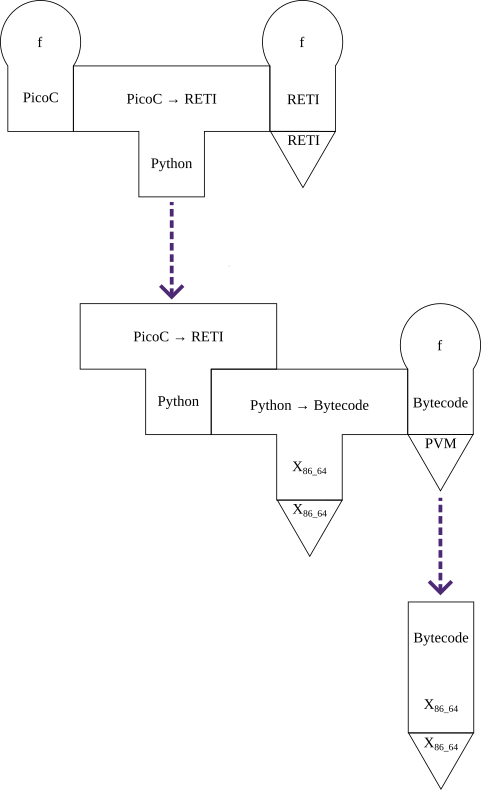
\includegraphics[width=0.5\linewidth]{./figures/summarized_cross_compiler.png}
  \caption{Cross-Compiler Kompiliervorgang ausgeschrieben}
  \label{fig:cross_compiler_kompiliervorgang_ausgeschrieben}
\end{figure}

Dieses längliche \colorbold{T-Diagram} in Abbildung~\ref{fig:cross_compiler_kompiliervorgang_ausgeschrieben} lässt sich zusammenfassen, sodass man das \colorbold{T-Diagram} in Abbildung~\ref{fig:cross_compiler_kompiliervorgang_kurzform} erhält, in welcher direkt angegeben ist, dass der \colorbold{PicoC-Compiler} in $\mathtt{X_{86\_64}}$-Maschienensprache geschrieben ist.

\begin{figure}[H]
  \centering
  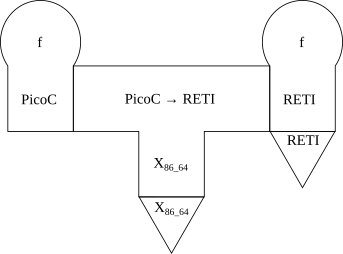
\includegraphics[width=0.33\linewidth]{./figures/compiliervorang_mit_machiene.png}
  \caption{Cross-Compiler Kompiliervorgang Kurzform}
  \label{fig:cross_compiler_kompiliervorgang_kurzform}
\end{figure}

Nachdem der Kompilierprozess des \colorbold{PicoC-Compiler} im \colorbold{vertikalen} nun genauer angesehen wurde, wird der Kompilierprozess im Folgenden im \colorbold{horinzontalen}, auf der Ebene der verschiedenen \colorbold{Passes} genauer betrachtet. Die Abbildung~\ref{fig:architektur_mit_allen_passes_ausgeschrieben} gibt einen guten Überblick über alle \colorbold{Passes} und wie diese in der \colorbold{Pipe-Architektur} (Definition~\ref{def:pipe_architektur}) des \colorbold{PicoC-Compilers} aufeinanderfolgen. In der \colorbold{Pipe-Architektur} nutzt der jeweils nächste \colorbold{Pass} den generierten \colorbold{Abstract Syntax Tree} des vorherigen Passes oder der Syntaktischen Analyse, um einen eigenen \colorbold{Abstract Syntax Tree} in seiner eigenen \colorbold{Sprache} zu generieren.

\begin{figure}[H]
  \centering
  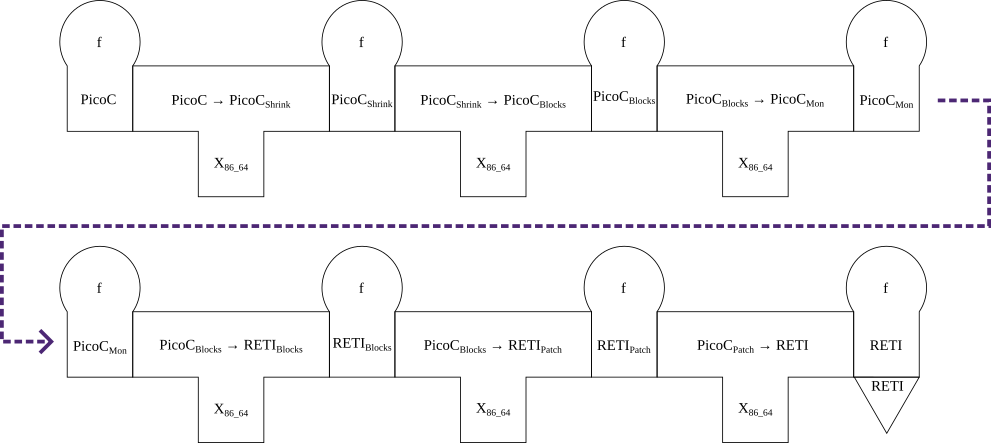
\includegraphics[width=\linewidth]{./figures/passes.png}
  \caption{Architektur mit allen Passes ausgeschrieben}
  \label{fig:architektur_mit_allen_passes_ausgeschrieben}
\end{figure}

Im Unterkapitel~\ref{sec:passes} werden die unterschiedlichen \colorbold{Passes} des PicoC-Compilers erklärt. In den darauffolgenden Unterkapiteln~\ref{sec:umsetzung_von_pointern},~\ref{sec:umsetzung_von_arrays},~\ref{sec:umsetzung_von_structs}~und~\ref{sec:umsetzung_von_funktionen} zu \colorbold{Pointern},  \colorbold{Arrays}, \colorbold{Structs} und \colorbold{Funktionen} werden einzelne \colorbold{Aspekte}, die Thema dieser \colorbold{Bachelorarbeit} sind \colorbold{genauer betrachtet} und erklärt, die im Unterkapitel~\ref{sec:passes} nicht ausreichend vertieft wurden. Viele der verwendenten \colorbold{Ansätze} zur Lösung dieser Probleme basieren auf der Vorlesung~\cite{scholl_betriebssysteme_2020} und wurden in dieser Bachelorarbeit weiter ausgearbeitet, wo es nötig war, sodass diese mit dem \colorbold{PicoC-Compiler} auch in der \colorbold{Praxis} implementiert werden konnten.

% https://tex.stackexchange.com/questions/167380/how-to-refer-to-a-footnote
Um die verschiedenen Aspekte besser erklären zu können, werden \colorbold{Codebeispiele} verwendet, in welchen ein kleines repräsentatives \colorbold{PicoC-Programm} für einen spezifischen Aspekt in wichtigen \colorbold{Zwischenstadien der Kompilierung} gezeigt wird\footnote{Also die verschiedenen in den \colorbold{Passes} generierten \colorbold{Abstract Syntax Trees}, sofern der \colorbold{Pass} für den gezeigten Aspekt relevant ist.}. Die \colorbold{Codebeispiele} wurden alle mit dem \colorbold{PicoC-Compiler} kompiliert und danach \colorbold{nicht} mehr \colorbold{verändert}, also genauso, wie der \colorbold{PicoC-Compiler} sie kompiliert aus den Dateien in dieses Dokument eingelesen. Alle hier zur Repräsentation verwendeten \colorbold{PicoC-Programme} lassen sich unter dem \footnoteurl{https://github.com/matthejue/Bachelorarbeit/tree/master/code_examples} finden und mithilfe der im Ordner \inlinebox{/code_examples} beiliegenden \inlinebox{Makefile} und dem Befehl \inlinebox*{make compile-all} genauso \colorbold{kompilieren}, wie sie hier dargestellt sind\footnote{Es wurden zu diesem Zweck spezielle neue \colorbold{Command-line Optionen} erstellt, die bestimmte Kommentare \colorbold{herausfiltern} und manche Container-Knoten \colorbold{einzeilig} machen, damit die generierten \colorbold{Abstract Syntax Trees} in den verscchiedenen Zwischenstufen der Kompilierung \colorbold{nicht} zu langgestreckt und \colorbold{überfüllt} mit Kommentaren sind.}.


\subsection{Passes}
\label{sec:passes}

Im Folgenden werden die verschiedenen \colorbold{Passes} des \colorbold{PicoC-Compilers} für die Generierung von \colorbold{RETI-Code} besprochen. Viele dieser \colorbold{Passes} haben \colorbold{Aufgaben}, die eher unter die Themenbereiche des \colorbold{Bachelorprojekts} fallen. Allerdings ist das Verständnis der \colorbold{Passes} auch für das Verständnis der veschiedenen Aspekte\footnote{In kurz: \colorbold{Pointer}, \colorbold{Arrays}, \colorbold{Strcuts} und \colorbold{Funktionen}.} der \colorbold{Bachelorarbeit} wichtig.

Auf jedes Detail der einzelnen \colorbold{Passes} wird in diesem Unterkapitel allerdings nicht eingegangen, da diese einerseits in den Unterkapiteln~\ref{sec:umsetzung_von_pointern},~\ref{sec:umsetzung_von_arrays},~\ref{sec:umsetzung_von_structs}~und~\ref{sec:umsetzung_von_funktionen} zu \colorbold{Pointern},  \colorbold{Arrays}, \colorbold{Structs} und \colorbold{Funktionen} im Detail erklärt sind und andererseits viele Aufgaben dieser \colorbold{Passes} eher dem \colorbold{Bachelorprojekt} zuzurechnen sind.

\subsubsection{PicoC-Shrink Pass}
\label{picoc_shrink_pass}
\newlineparagraph{Aufgabe}
\label{sec:picoc_shrink_pass_zweck}
% dieser Pass existiert nur wegen der Erweiterungen

Der Aufgabe des \colorbold{PicoC-Shrink Pass} ist in Unterkapitel~\ref{dereferenzierung_durch_zugriff_auf_arrayindex_ersetzen} ausführlich an einem Beispiel erklärt. Kurzgefasst hat der \colorbold{PicoC-Shrink Pass} die Aufgabe, die Eigenheit auszunutzen, dass der \colorbold{Dereferenzierungoperator} \smalltt{*pntr} und die damit einhergehende \colorbold{Pointer Arithmetik} \smalltt{*(pntr + i)} sich in der Untermenge der Sprache $L_{C}$, welche die Sprache $L_{PicoC}$ darstellt genau gleich verhält, wie der \colorbold{Operator} für den \colorbold{Zugriff} auf den \colorbold{Index} eines \colorbold{Arrays} \smalltt{ar[i]}.

Daher wandelt der \colorbold{PicoC-Shrink Pass} alle Verwendungen des \colorbold{Knoten} \smalltt{Deref(exp, i)} im jeweiligen \colorbold{Abstract Syntax Tree} in \colorbold{Knoten} \smalltt{Subscr(exp, i)} um, sodass sich dadurch viele vermeidbare \colorbold{Fallunterscheidungen} und \colorbold{doppelter Code} bei der Implementierung sparren lassen, denn man kann die \colorbold{Derefenzierung} \smalltt{*(var + i)} einfach von den Routinen für einen \colorbold{Zugriff auf einen Arrayindex} \smalltt{var[i]} übernehmen lassen.

\newlineparagraph{Codebeispiel}

In den nächsten Unterkapiteln wird das Beispiel in Code~\ref{code:picoc_code_für_codebeispiel} zur \colorbold{Anschauung} der verschiedenen \colorbold{Passes} verwendet. Im Code~\ref{code:picoc_code_für_codebeispiel} ist in der Funktion \smalltt{faculty} ein \colorbold{iterativer} Algorithmus implementiert, der die \colorbold{Fakultät} eines übergebenen \colorbold{Arguments} berechnet. Der Algorithmus basiert auf einem \colorbold{Beispielprogramm} aus der Vorlesung~\cite{scholl_betriebssysteme_2020}, der in der Vorlesung allerdings \colorbold{rekursiv} implementiert war.
% natürlich beide Beispiele als Tests verfügbar

Dieser \colorbold{rekursive} Algoirthmus ist allerdings \colorbold{kein} gutes \colorbold{Anschaungsbeispiel}, dass viele der Aufgaben der verschiedenen \colorbold{Passes} bei der Kompilierung veranschaulicht hätte. Viele Aufgaben der \colorbold{Passes}, wie z.B. bei der Kompilierung von \smalltt{if}-, \smalltt{if-else}-, \smalltt{while}- und \smalltt{do-while}-Statements wären im Beispiel aus der Vorlesung \colorbold{nicht} enthalten gewesen. Daher wurde das Beispiel aus der Vorlesung zu einem \colorbold{iterativen} Algorithmus~\ref{code:picoc_code_für_codebeispiel} umgeschrieben, um \smalltt{if}- und \smalltt{while}-Statemtens zu enthalten.

Beide Varianten des Algorithmus wurden zum Testen des \colorbold{PicoC-Compilers} verwendet und sind als Tests im Ordner \inlinebox{/tests} unter \footnoteurl{https://github.com/matthejue/PicoC-Compiler/tree/new_architecture/tests} unter den Testbezeichnungen \inlinebox{example_faculty_rec.picoc} und \inlinebox{example_faculty_it.picoc} zu finden.

Die Codebeispiele in diesem und den folgenden Unterkapiteln dienen allerdings nur als \colorbold{Anschauung} des jeweiligen \colorbold{Passes}, der in diesem Unterkapitel beschrieben wird und werden nicht im Detail erläutert, da viele Details der Passes später in den Unterkapiteln~\ref{sec:umsetzung_von_pointern},~\ref{sec:umsetzung_von_arrays},~\ref{sec:umsetzung_von_structs}~und~\ref{sec:umsetzung_von_funktionen} zu \colorbold{Pointern},  \colorbold{Arrays}, \colorbold{Structs} und \colorbold{Funktionen} mit eigenen \colorbold{Codebeispielen} erklärt werden und alle sonstigen Details dem \colorbold{Bachelorprojekt} zuzurechnen sind.

\begin{code}
  \centering
  \numberedcodebox[minted language=c]{./code_examples/example_faculty_it.picoc}
  \caption{PicoC Code für Codebespiel}
  \label{code:picoc_code_für_codebeispiel}
\end{code}

In Code~\ref{code:abstract_syntax_tree_für_codebeispiel} sieht man den \colorbold{Abstract Syntax Tree}, der in der \colorbold{Syntaktischen Analyse} generiert wurde.

\begin{code}
  \centering
  \numberedcodebox[minted language=text]{./code_examples/example_faculty_it.ast}
  \caption{Abstract Syntax Tree für Codebespiel}
  \label{code:abstract_syntax_tree_für_codebeispiel}
\end{code}

Im \colorbold{PicoC-Shrink-Pass} ändert sich nichts im Vergleich zum \colorbold{Abstract Syntax Tre} in Code~\ref{code:abstract_syntax_tree_für_codebeispiel}, da das Codebeispiel keine \colorbold{Dereferenzierung} enthält.

% TODO: nichts hinzugefügt zu Syntax

\subsubsection{PicoC-Blocks Pass}
\label{picoc_blocks_pass}
\newlineparagraph{Aufgabe}
\label{sec:picoc_blocks_pass_zweck}

Die Aufgabe des \colorbold{PicoC-Blocks Passes} ist die Knoten \smalltt{If(exp, stmts)}, \smalltt{IfElse(exp, stmts1, stmts2)}, \smalltt{While(exp, stmts)} und \smalltt{DoWhile(exp, stmts)} mithilfe von \smalltt{Block(name, stmts\_instrs}-, \smalltt{GoTo(lable)}- und \smalltt{IfElse(exp, stmts1, stmts2)}-Knoten umzusetzen. Der \smalltt{IfElse(exp, stmts1, stmts2)}-Knoten wird zur Umsetzung der \colorbold{Bedingung} verwendet und es wird, je nachdem, ob die Bedingung \colorbold{wahr} oder \colorbold{falsch} ist mithilfe der \smalltt{GoTo(label)}-Knoten in einen von zwei \colorbold{alternativen Branches} gesprungen oder ein \colorbold{Branch} erneut aufgerufen usw.

\newlineparagraph{Abstrakte Syntax}

Zur Umsetzung dieses Passes ist es notwendig die \colorbold{Abstrakte Syntax}~\ref{gr:abstract_syntax_l_picoc} um die Knoten zu erweitern, die im Unterkapitel \ref{sec:picoc_blocks_pass_zweck} erwähnt wurden. Des Weiteren wird für die \colorbold{Kommentare}, die in vielen Codebeispielen zur leichteren Verständlichkeit eingefügt wurden ein \smalltt{SingleLineComment(prefix, content)}-Knoten benötigt. Die \colorbold{Funktionsdefinition} \smalltt{FunDef(⟨datatype⟩, Name(str), L Fun Alloc(Writeable(), ⟨datatype⟩, Name(str))*, ⟨block⟩*)} ist nun ein Container für \colorbold{Blöcke} \smalltt{Block(Name(str), ⟨stmt⟩*)} und keine Statements \smalltt{stmt} mehr.

\begin{grammar}[Abstrakte Syntax für $L_{PicoC\_Blocks}$][H][gr:abstract_syntax_l_picoc_blocks]
  \toprule
  \firstcase{decl\_def}{FunDef(\langle datatype\rangle , Name(str),}{L\_Fun}
  & & \qquad $Alloc(Writeable(), \langle datatype\rangle , Name(str))*, \langle block\rangle *)$ & \\
  \midrule
  \firstcase{block}{Block(Name(str), \langle stmt\rangle *)}{L\_Blocks}
  \firstcase{stmt}{GoTo(Name(str)) \gralt SingleLineComment(str, str)}{}
  \bottomrule
\end{grammar}


% man tut so als gäbe es Konkrette Syntax

\newlineparagraph{Codebeispiel}

In Code~\ref{code:picoc_blocks_pass_für_codebeispiel} sieht man den \colorbold{Abstract-Syntax-Tree} des \colorbold{PiocC-Blocks Passes} für das aus Unterkapitel~\ref{code:picoc_code_für_codebeispiel} weitergeführte Beispiel, indem nun eigene \colorbold{Blöcke} für die Funktion \smalltt{faculty} und die \smalltt{main}-Funktion erstellt werden, in denen die \colorbold{ersten} Statements der jeweiligen Funktionen bis zu \colorbold{letzten} Statement oder bis zum ersten \colorbold{Auftauchen} eines \smalltt{If(exp, stmts)}-, \smalltt{IfElse(exp, stmts1, stmts2)}-, \smalltt{While(exp, stmts)}- oder \smalltt{DoWhile(exp, stmts)}-Knoten stehen. Je nachdem, ob ein \smalltt{If(exp, stmts)}-, \smalltt{IfElse(exp, stmts1, stmts2)}-, \smalltt{While(exp, stmts)}- oder \smalltt{DoWhile(exp, stmts)}-Knoten auftaucht, werden für die \colorbold{Bedingung} und mögliche \colorbold{Branches} eigene \colorbold{Blöcke} erstellt.

\begin{code}
  \centering
  \numberedcodebox[minted language=text]{./code_examples/example_faculty_it.picoc_blocks}
  \caption{PicoC-Blocks Pass für Codebespiel}
  \label{code:picoc_blocks_pass_für_codebeispiel}
\end{code}

\subsubsection{PicoC-Mon Pass}
\label{picoc_mon_pass}
\newlineparagraph{Aufgabe}
\label{sec:picoc_mon_pass_zweck}

Die Aufgabe des \colorbold{PicoC-Mon Pass} ist es den \colorbold{Abstract Syntax Tree} \dq in eine \colorbold{eingeschränkte Form} zu bringen, in der die \colorbold{Argumente} von \colorbold{Operationen} \colorbold{Atomare Audrücke} sind\dq\footcite{g_siek_course_2022}

\newlineparagraph{Abstrakte Syntax}
\begin{grammar}[Abstrakte Syntax für $L_{PicoC\_Mon}$][H][gr:abstract_syntax_l_picoc_mon]
  \toprule
  \firstcase{ref\_loc}{Stack(Num(str)) \gralt Global(Num(str))}{L\_Assign\_Alloc}
  \otherform{Stackframe(Num(str))}{}
  \firstcase{error\_data}{\langle exp\rangle  \gralt Pos(Num(str), Num(str))}{}
  \firstcase{exp}{Stack(Num(str)) \gralt Ref(\langle ref_loc\rangle , \langle datatype\rangle , \langle error_data\rangle )}{}
  \firstcase{stmt}{Exp(\langle exp\rangle )}{}
  \otherform{Assign(Alloc(Writeable(), StructSpec(Name(str)), Name(str)), }{}
  & & \qquad $Struct(Assign(Name(str), \langle exp\rangle )+, \langle datatype\rangle$ )) & \\
  \otherform{Assign(Alloc(Writeable(), ArrayDecl(Num(str)+, \langle datatype\rangle ),}{}
  & & \qquad $Name(str)), Array(\langle exp\rangle +, \langle datatype\rangle ))$ & \\
  \otherform{NewStackframe(Name(), GoTo(str))}{}
  \otherform{RemoveStackframe()}{}
  \midrule
  \firstcase{symbol\_table}{SymbolTable(\langle symbol\rangle )}{L\_Symbol\_Table}
  \firstcase{symbol}{Symbol(\langle type_qual\rangle , \langle datatype\rangle , \langle name\rangle , \langle val\rangle , \langle pos\rangle , \langle size\rangle )}{}
  \firstcase{type\_qual}{Empty()}{}
  \firstcase{datatype}{BuiltIn() \gralt SelfDefined()}{}
  \firstcase{name}{Name(str)}{}
  \firstcase{val}{Num(str) \gralt Empty()}{}
  \firstcase{pos}{Pos(Num(str), Num(str)) \gralt Empty()}{}
  \firstcase{size}{Num(str) \gralt Empty()}{}
  \bottomrule
\end{grammar}

\begin{Definition}{Symboltabelle}{symboltabelle}
\end{Definition}

\newlineparagraph{Codebeispiel}

\begin{code}
  \centering
  \numberedcodebox[minted language=text]{./code_examples/example_faculty_it.picoc_mon}
  \caption{PicoC-Mon Pass für Codebespiel}
  \label{code:picoc_mon_pass_für_codebeispiel}
\end{code}

\subsubsection{RETI-Blocks Pass}
\label{reti_blocks_pass}
\newlineparagraph{Aufgaben}
\label{sec:reti_blocks_pass_zweck}
\newlineparagraph{Abstrakte Syntax}
\begin{grammar}[Abstrakte Syntax für $L_{RETI\_Blocks}$][H][gr:abstract_syntax_l_reti_blocks]
  \toprule
  \firstcase{program}{Program(Name(str), \langle block\rangle *)}{L\_Program}
  \midrule
  \firstcase{exp\_stmts}{GoTo(str)}{L\_Blocks}
  \firstcase{instrs\_before}{Num(str)}{}
  \firstcase{num\_instrs}{Num(str)}{}
  \firstcase{block}{Block(Name(str), \langle instr\rangle *, \langle instrs\_before\rangle , \langle num\_instrs\rangle )}{}
  \firstcase{instr}{GoTo(Name(str))}{}
  \bottomrule
\end{grammar}

\newlineparagraph{Codebeispiel}

\begin{code}
  \centering
  \numberedcodebox[minted language=text]{./code_examples/example_faculty_it.reti_blocks}
  \caption{RETI-Blocks Pass für Codebespiel}
  \label{code:reti_blocks_pass_für_codebeispiel}
\end{code}

\subsubsection{RETI-Patch Pass}
\label{reti_patch_pass}
\newlineparagraph{Aufgaben}
\label{sec:reti_patch_pass_zweck}
\newlineparagraph{Abstrakte Syntax}
\begin{grammar}[Abstrakte Syntax für $L_{RETI\_Patch}$][H][gr:abstract_syntax_l_reti_patch]
  \toprule
  \firstcase{stmt}{Exit(Num(str))}{}
  \bottomrule
\end{grammar}

\newlineparagraph{Codebeispiel}

\begin{code}
  \centering
  \numberedcodebox[minted language=text]{./code_examples/example_faculty_it.reti_patch}
  \caption{RETI-Patch Pass für Codebespiel}
  \label{code:reti_patch_pass_für_codebeispiel}
\end{code}

\subsubsection{RETI Pass}
\label{reti_pass}
\newlineparagraph{Aufgaben}
\label{sec:reti_pass_zweck}
\newlineparagraph{Konkrette und Abstrakte Syntax}

% dieser Pass entspricht Assembler bis auf die Sache mit binärer Repräsentation, was der PicoC-Compiler garnicht macht

\begin{grammar}[Konkrette Syntax für $L_{RETI\_Lex}$][H][gr:konkrette_syntax_l_reti_lexer]
\toprule
\firstcase{dig\_no\_0}{ \dq 1\dq \gralt \dq 2\dq \gralt \dq 3\dq \gralt \dq 4\dq \gralt \dq 5\dq \gralt \dq 6\dq}{L\_Program}
\otherform{\dq 7\dq \gralt \dq 8\dq \gralt \dq 9\dq}{}
\firstcase{dig\_with\_0}{ \dq 0\dq \gralt dig\_no\_0}{}
\firstcase{num}{ \dq 0\dq \gralt dig\_no\_0dig\_with\_0*\gralt \dq {-}\dq dig\_with\_0*}{}
\firstcase{letter}{ \dq a\dq ... \dq Z\dq }{}
\firstcase{name}{ letter(letter \mid  dig\_with\_0 \mid  \_)*}{}
\firstcase{reg}{ \dq ACC\dq \gralt \dq IN1\dq \gralt \dq IN2\dq \gralt \dq PC\dq \gralt \dq SP\dq}{}
\otherform{\dq BAF\dq \gralt \dq CS\dq \gralt \dq DS\dq}{}
\firstcase{arg}{ reg \gralt  num}{}
\firstcase{rel}{ \dq {==}\dq \gralt \dq {!=}\dq \gralt \dq {<}\dq \gralt \dq {<=}\dq\gralt \dq {>}\dq}{}
\otherform{\dq {>=}\dq \gralt \dq \_NOP\dq}{}
\bottomrule
\end{grammar}

\begin{grammar}[Konkrette Syntax für $L_{RETI\_Parse}$][H][gr:konkrette_syntax_l_reti_parser]
\toprule
\firstcase{instr}{\dq ADD\dq\enspace reg\enspace arg\gralt \dq ADDI\dq\enspace reg\enspace num\gralt \dq SUB\dq\enspace reg\enspace arg}{L\_Program}
\otherform{\dq SUBI\dq\enspace reg\enspace\enspace num\gralt \dq MULT\dq\enspace reg\enspace arg\gralt \dq MULTI\dq\enspace reg\enspace num}{}
\otherform{\dq DIV\dq\enspace reg\enspace arg\gralt \dq DIVI\dq\enspace reg\enspace num\gralt \dq MOD\dq\enspace reg\enspace arg}{}
\otherform{\dq MODI\dq\enspace reg\enspace num\gralt \dq OPLUS\dq\enspace reg\enspace arg\gralt \dq OPLUSI\dq\enspace reg\enspace num}{}
\otherform{\dq OR\dq\enspace reg\enspace arg\gralt \dq ORI\dq\enspace reg\enspace num}{}
\otherform{\dq AND\dq\enspace reg\enspace arg\gralt \dq ANDI\dq\enspace reg\enspace num}{}
\otherform{\dq LOAD\dq\enspace reg\enspace num\gralt \dq LOADIN\dq\enspace arg\enspace arg\enspace num}{}
\otherform{\dq LOADI\dq\enspace reg\enspace num}{}
\otherform{\dq STORE\dq\enspace reg\enspace num\gralt \dq STOREIN\dq\enspace arg\enspace arg num}{}
\otherform{\dq MOVE\dq\enspace reg\enspace reg}{}
\otherform{\dq JUMP\dq rel\enspace num\gralt INT\enspace num\gralt RTI}{}
\otherform{\dq CALL\dq\enspace \dq INPUT\dq\enspace  reg\gralt \dq CALL\dq\enspace \dq PRINT\dq\enspace reg}{}
\firstcase{program}{name\enspace (instr\dq ;\dq )*}{}
\bottomrule
\end{grammar}

% TODO: es braucht noch eine Konkrette Syntax dafür
\begin{grammar}[Abstrakte Syntax für $L_{RETI}$][H][gr:abstract_syntax_l_reti]
  \toprule
  \firstcase{reg}{ACC() \gralt IN1() \gralt IN2() \gralt PC() \gralt SP() \gralt BAF()}{L\_Program}
  \otherform{CS() \gralt DS()}{}
  \firstcase{arg}{Reg(\langle reg\rangle ) \gralt Num(str)}{}
  \firstcase{rel}{Eq() \gralt NEq() \gralt Lt() \gralt LtE() \gralt Gt() \gralt GtE()}{}
  \otherform{Always() \gralt NOp()}{}
  \firstcase{op}{Add() \gralt Addi() \gralt Sub() \gralt Subi() \gralt Mult()}{}
  \otherform{Multi() \gralt Div() \gralt Divi()}{}
  \otherform{Mod() \gralt Modi() \gralt Oplus() \gralt Oplusi() \gralt Or()}{}
  \otherform{Ori() \gralt And() \gralt Andi()}{}
  \otherform{Load() \gralt Loadin() \gralt Loadi()}{}
  \otherform{Store() \gralt Storein() \gralt Move()}{}
  \firstcase{instr}{Instr(\langle op\rangle , \langle arg\rangle +) \gralt Jump(\langle rel\rangle , Num(str)) \gralt Int(Num(str))}{}
  \otherform{RTI() \gralt Call(Name('print'), \langle reg\rangle ) \gralt Call(Name('input'), \langle reg\rangle )}{}
  \otherform{SingleLineComment(str, str)}{}
  \firstcase{program}{Program(Name(str), \langle instr\rangle *)}{}
  \bottomrule
\end{grammar}

\newlineparagraph{Codebeispiel}

\begin{code}
  \centering
  \numberedcodebox[minted language=text]{./code_examples/example_faculty_it.reti}
  \caption{RETI Pass für Codebespiel}
  \label{code:reti_pass_für_codebeispiel}
\end{code}

% TODO: zusammenfassendes Bild
